\documentclass[no-math,10pt]{ctexbook}
%空心句号自动转化为实心点号
\defaultfontfeatures{Mapping=fullwidth-stop}
%思源字体标宋
\setCJKfamilyfont{zhbs}{Source Han Serif CN Bold}% 标song
\def\bs{\CJKfamily{zhbs}}
%开明标点制,全文宋体标点,数学模式直接输入中文,避免孤字成行
\xeCJKsetup{PunctStyle=kaiming,PunctFamily=zhsong,CJKmath,CheckSingle}
%设置英文字体
\setmainfont[BoldFont=Times New Roman-Bold,BoldItalicFont=Times New Roman-Bold Italic]{CMU Serif}
\setsansfont{Arial}
\setmonofont{CMU Typewriter Text}
%数学宏包
\usepackage{mathtools,amssymb,mathrsfs,empheq,scalerel,esvect,zhmathstyle,mathsymbolzhcn}
\let\leq\leqslant
\let\geq\geqslant
%数学字体尺寸
\DeclareMathSizes{10.5bp}{10.5bp}{6.8pt}{6pt}
\allowdisplaybreaks[4]
\usepackage{zhshuzi}
  \usepackage{geometry}
\geometry{paperheight=29.7cm,
	paperwidth=21cm,
	width=17cm,
	height=24.7cm,
	left=1.8cm,
	right=1.6cm,
	top=2.5cm,
	bottom=2.5cm,
	headsep=3.2em,
	marginparsep=-13.5em,
	marginparwidth=13em,
	reversemarginpar}

\usepackage{tikz,tikzpagenodes}
\usetikzlibrary{shapes.callouts,shapes.geometric,positioning}
\newcommand{\lanmu}[1]{
\begin{center}
	\begin{tikzpicture}
	\node[cloud callout, cloud puffs=15, aspect=4.5, cloud puff arc=120,
	draw,text=black,font=\bs\Large,shading=ball,ball color=gray!20] at(0,0){#1};
	\end{tikzpicture}
\end{center}
}


\usepackage[most]{tcolorbox}

\usepackage{varwidth}
\newtcolorbox{xxmb}[1][]{nobeforeafter,valign=center,enhanced,width=0.495\textwidth,
	colback=white,colframe=gray!70!black,sharp corners=east,arc is angular,arc=2mm,leftrule=0mm,,bottom=0mm,
	attach boxed title to top center={xshift=0.29cm,yshift*=1mm-\tcboxedtitleheight},
	varwidth boxed title*=-3cm,
	boxed title style={frame code={
			\path[fill=gray!70!black]
			([yshift=-1mm,xshift=-1mm]frame.north west)
			arc[start angle=0,end angle=180,radius=1mm]
			([yshift=-1mm,xshift=1mm]frame.north east)
			arc[start angle =180,end angle=0,radius=1mm];
			\path[fill,gray!70!black]
			([xshift=-2mm]frame.north west) -- ([xshift=2mm]frame.north east)
			[rounded corners=1mm]-- ([xshift=1mm,yshift=-1mm]frame.north east)
			-- (frame.south east) -- (frame.south west)
			-- ([xshift=-1mm,yshift=-1mm]frame.north west)
			[sharp corners]-- cycle;
		},interior engine=empty,
	},
	fonttitle=\zihao{4}\bfseries,
	title={学习目标},height=#1 cm}
\newtcolorbox{zdnd}[1][]{left skip=-1mm,nobeforeafter,valign=center,enhanced,width=0.495\textwidth,
	colback=white,colframe=gray!70!black,sharp corners=west,arc is angular,arc=2mm,rightrule=0mm,bottom=0mm,
	attach boxed title to top center={xshift=0.29cm,yshift*=1mm-\tcboxedtitleheight},
	varwidth boxed title*=-3cm,
	boxed title style={frame code={
			\path[fill=gray!70!black]
			([yshift=-1mm,xshift=-1mm]frame.north west)
			arc[start angle=0,end angle=180,radius=1mm]
			([yshift=-1mm,xshift=1mm]frame.north east)
			arc[start angle =180,end angle=0,radius=1mm];
			\path[fill,gray!70!black]
			([xshift=-2mm]frame.north west) -- ([xshift=2mm]frame.north east)
			[rounded corners=1mm]-- ([xshift=1mm,yshift=-1mm]frame.north east)
			-- (frame.south east) -- (frame.south west)
			-- ([xshift=-1mm,yshift=-1mm]frame.north west)
			[sharp corners]-- cycle;
		},interior engine=empty,
	},
	fonttitle=\zihao{4}\bfseries,
	title={重点难点},height=#1 cm}
\usepackage{enumitem}
\setenumerate{itemsep=0pt,partopsep=0pt,parsep=\parskip,topsep=0pt}
\setenumerate[2]{align=left,label=({\makebox[0.8em]{\arabic*}}),labelwidth=1.7em,labelsep=0em,leftmargin=1.7em}
 \newenvironment{mubiao}{
	\begin{enumerate}[label=\arabic*.,align=left,labelindent=0em,
labelwidth=1em,labelsep=0em,leftmargin=1em]\fangsong}{\end{enumerate}}
\setdescription{itemsep=0pt,partopsep=0pt,parsep=\parskip,topsep=0pt}
\newenvironment{zndian}{
	\begin{description}[align=left,labelindent=0em,
		labelwidth=3em,labelsep=0em,leftmargin=3em,font=\bf]
	\fangsong}{\end{description}}


%对位环境
\RequirePackage{hlist}
\newenvironment{xx}[5][4]{
	\begin{hlist}[pre skip=0pt,post skip=0pt,label=\Alpha{hlisti}.,pre label=,item offset=1.2em,col sep=0.5em]#1
		\hitem #2 \hitem #3 \hitem #4 \hitem #5
	}{\end{hlist}}
\newenvironment{tg}[5][4]{
	\begin{hlist}[pre skip=0pt,post skip=0pt,show label= false,pre label=,item offset=1.2em,col sep=0.5em]#1
		\hitem #2 \hitem #3 \hitem #4 \hitem #5
	}{\end{hlist}}

%变式练习
\usepackage{bbding}
\newcounter{bianshi}
\newenvironment{bslx}{\HandPencilLeft\fbox{\bf\thesubsubsection 对接练习}\begin{enumerate}[labelindent=0mm,align=left,labelwidth=1em,labelsep=0em,leftmargin=1em,label={\bf\arabic*.}]
	}{\end{enumerate}}
%方法归纳
\newtcolorbox{ffgn}{enhanced,breakable,boxrule=0.5mm,title={\bf 方法归纳},left=0pt,top=2mm,bottom=0mm,colframe=black,parbox=false,arc is angular,arc=1mm,fontupper=\indent\kaishu,
	colback=gray!10,colbacktitle=gray,coltitle=white,attach boxed title to top center=
	{yshift=-0.25mm-\tcboxedtitleheight/2,yshifttext=2mm-\tcboxedtitleheight/2},
	boxed title style={boxrule=0.5mm,
		frame code={ \path[fill=black] ([xshift=-4mm]frame.west)
			-- (frame.north west) -- (frame.north east) -- ([xshift=4mm]frame.east)
			-- (frame.south east) -- (frame.south west) -- cycle; },
		interior code={ \path[tcb fill interior] ([xshift=-2mm]interior.west)
			-- (interior.north west) -- (interior.north east)
			-- ([xshift=2mm]interior.east) -- (interior.south east) -- (interior.south west)
			-- cycle;}}
}
%校本作业
\newenvironment{zuoye}{\begin{enumerate}[labelindent=0mm,align=left,labelwidth=1.5em,labelsep=0em,leftmargin=1.5em,label={\hquan{\arabic*}},series=zuoye,resume=zuoye]
	}{\end{enumerate}}

 \usepackage{multicol}
\usepackage[tikz]{multicolrule}
\usetikzlibrary{decorations.pathmorphing}
\setlength{\columnsep}{2em}
\SetMCRule{width=0.5pt,
	custom-line={
		\draw[decorate,decoration={coil,aspect=0}] (TOP)--(BOT);
}}
\usepackage{float}
\makeatletter
\newenvironment{tablehere}
{\def\@captype{table}}
{}

\newenvironment{figurehere}
{\def\@captype{figure}}
{}
\makeatother
\usepackage{graphicx}
\usepackage{caption}
\captionsetup{labelsep=quad,font=rm,font=small,aboveskip=6pt}
\renewcommand{\thefigure}{\thechapter{}-\arabic{figure}}
\renewcommand{\thetable}{\thechapter{}-\arabic{table}}
%\captionsetup[table]{position=above}
 %数学间距
\lineskiplimit=5pt
\lineskip=6pt
\thinmuskip=2mu
\medmuskip=3mu plus  1mu minus 2mu
\thickmuskip=3mu plus 2mu
%定界符高度
\delimiterfactor=800
	%正文行距
\usepackage[bodytextleadingratio=1.5,restoremathleading=true]{zhlineskip}
\SetMathEnvironmentSinglespace{1.1}
%章节标题
\usepackage{fontawesome,etoolbox}
\setcounter{secnumdepth}{3}
\usepackage[explicit,indentafter,pagestyles]{titlesec}

\newcounter{countchapters}

\newif\ifmulticolsused

\pretocmd{\multicols}{\global\multicolsusedtrue}{}{}
\apptocmd{\endmulticols}{\global\multicolsusedfalse}{}{}

% From http://tex.stackexchange.com/questions/199139
\titleformat{\chapter}
{\Huge\bfseries}
{}
{0em}{\begin{tikzpicture}[remember picture,overlay]
	\fill[gray!30](current page.north west)[rounded corners=3cm]--++(1cm,-4cm)[rounded corners=0cm]--([yshift=-4cm]current page.north east)--(current page.north east)--cycle;
	\node[circular sector,circular sector angle=110,shape border rotate=90,fill=black!70,right,text=white,font=\bf\huge,inner sep=20pt]at([shift={(2cm,-2cm)}]current page.north west){\CTEXthechapter};
	\node[inner sep=0mm,font=\bf\huge,anchor= west]at([shift={(10cm,-2.5cm)}]current page.north west){#1};
	\end{tikzpicture}
}
[\ifnum\value{chapter}>0 
\addtocontents{toc}{\protect\begin{multicols}{2}\protect\multicolsusedtrue}
	\fi
	\stepcounter{countchapters}
	]
	
	\titleformat{name=\chapter,numberless}
	{\Huge\bfseries}
	{}
	{0em}{
		\begin{tikzpicture}[remember picture,overlay]
		\draw[line width=1.2pt]([yshift=-3cm]current page.north east)--++(-6cm,0);
		\node at([shift={(-4.5cm,-2.5cm)}]current page.north east){#1};
		\node at([shift={(-4.5cm,-3.5cm)}]current page.north east){Contents};
		\end{tikzpicture}
		}[]
	\titlespacing*{\chapter}{0em}{0em}{1em}
	\pretocmd{\chapter}{%
		% Close the multicols if needed
		\addtocontents{toc}{\protect\ifmulticolsused\protect\end{multicols}\protect\fi}
}{}{}

\AtEndDocument{%
	% Close the multicols if needed
	\addtocontents{toc}{\protect\ifmulticolsused\protect\end{multicols}\protect\fi}
}




\titleformat{\section}
{\bf\LARGE\centering}
{\faBook~\thesection}
{1em}
{#1}
[]


\renewcommand{\thesubsubsection}{题型\arabic{subsubsection}}
\titleformat{\subsubsection}
{\bf\large}
{}
{0em}
{\begin{tcolorbox}[nobeforeafter,width=0.5\textwidth-1em,arc=0mm,enhanced,bicolor,colback=gray!70!black,colbacklower=gray!20,sidebyside,lefthand ratio=0.17,sidebyside gap=1mm,left=0.5mm,halign=left,fontupper=\color{white},boxrule=0mm,top=1mm,bottom=1mm]\thesubsubsection\tcblower#1\end{tcolorbox}}
[]
\titlespacing*{\subsubsection}{0pt}{0em}{0em}

\setcounter{tocdepth}{3}


\renewcommand{\contentsname}{目\quad 录}
\usepackage[titles]{tocloft}
\renewcommand{\cftdot}{\Large$\cdot$}
\renewcommand{\cftdotsep}{0.9}

\renewcommand{\cftsecpagefont}{\large}
\renewcommand{\cftsecfont}{\large}
\renewcommand{\cftsecindent}{0em}
\renewcommand{\cftbeforesecskip}{0.3em}
\renewcommand{\cftsubsecfont}{\large}
\renewcommand{\cftsubsecindent}{2.5em}
\renewcommand{\cftbeforesubsecskip}{0.3em}
\renewcommand{\cftsubsecpagefont}{\large}
\renewcommand{\cftsubsubsecfont}{\fangsong}
\renewcommand{\cftsubsubsecindent}{2.3em}
\renewcommand{\cftsubsubsecnumwidth}{3em}
\usepackage{titletoc}
\titlecontents{chapter}[0em]
{\large\filcenter}
{\bf\thecontentslabel}{}
{}
[{\titlerule[1pt]\addvspace{1em}}]

\usepackage{zhlipsum,calc}
\newzhlipsum{mingyan}
{
	{阅读使人充实,会谈使人敏捷,写作使人精确。——培根},
	{知人者智,自知者明。胜人者有力,自胜者强。——老子},
	{阅读使人充实,会谈使人敏捷,写作使人精确。——培根},
	{业精于勤,荒于嬉;行成于思,毁于随。——韩愈},
	{敏而好学,不耻下问。——孔子},
	{海纳百川有容乃大;壁立千仞无欲则刚。——林则徐},
	{穷则独善其身,达则兼济天下。——孟子},
	{读书破万卷,下笔如有神。——杜甫},
	{君子之交淡若水,小人之交甘若醴,君子淡以亲,小人甘以绝。——庄子},
	{三更灯火五更鸡,正是男儿读书时,黑发不知勤学早,白首方悔读书迟。——颜真卿},
}
  \newpagestyle{math}
{   
	\sethead[
	\begin{tikzpicture}[remember picture,overlay]
	\draw([xshift=1.5cm,yshift=1cm]current page header area.south west)--([xshift=1.5cm]current page header area.south west)--++(7cm,0);
	\node[anchor=south west,rectangle callout,callout relative pointer={(-25:0.5)},inner sep=1em,fill=gray,text=white,font=\sf\large] at(current page header area.south west){\thepage};
	\node[anchor=west]at([xshift=1.6cm,yshift=0.3cm]current page header area.south west){导学案第一册};
	\end{tikzpicture}
	][][]
	{\begin{tikzpicture}[remember picture,overlay]
		\draw([xshift=-1.5cm,yshift=1cm]current page header area.south east)--([xshift=-1.5cm]current page header area.south east)--++(-7cm,0);
		\node[anchor=south east,inner sep=1em,,rectangle callout,callout relative pointer={(-155:0.5)},fill=gray,text=white,font=\sf\large] at(current page header area.south east){\thepage};
		\node[anchor=east]at([xshift=-1.6cm,yshift=0.3cm]current page header area.south east){\ifthechapter{\CTEXthechapter~\chaptertitle}{\chaptertitle}};
		\end{tikzpicture}}{}{}
	\setfoot[\ifthechapter{
	\begin{tikzpicture}[remember picture,overlay]
	\fill[gray!20]([yshift=-1.5cm]current page footer area.south west) rectangle (current page footer area.north east);
	\node[anchor=west,font=\kaishu]at([yshift=-2em]current page footer area.west)
	{\parbox{\textwidth-5mm}{\CTEXindent\zhlipsum[\thepage][name=mingyan]
		}};
	\end{tikzpicture}}{}
	][][]
	{\begin{tikzpicture}[remember picture,overlay]
		\fill[gray!20]([yshift=-1.5cm]current page footer area.south west) rectangle (current page footer area.north east);
		\node[anchor=west,font=\kaishu]at([yshift=-2em]current page footer area.west)
		{\parbox{\textwidth-5mm}{\CTEXindent\zhlipsum[\thepage][name=mingyan]}};
		\end{tikzpicture}
	}{}{}
}
\pagestyle{math}
\assignpagestyle{\chapter}{empty}


%例题环境
\newcounter{lt}[section]
\newenvironment{liti}{\refstepcounter{lt}
	\begin{enumerate}[align=left,labelindent=0mm,label={\bf\faCogs 例\fquan{\thelt}},labelwidth=3.8em,labelsep=0mm,leftmargin=3.8em]
		\item 
	}{\end{enumerate}}
%解析环境
\usepackage{comment}
\tcbset{jx/.style={breakable,enhanced,colback=white,colframe=white,height=1.7cm,
		overlay={\foreach \a in{-1.2,-2.8,-4.4}
			\draw[dashed]([shift={(3.2em,\a em)}]frame.north west)--([shift={(0,\a em)}]frame.north east);
			\node at([shift={(3.8em,-0.7em)}]frame.north west){\bf 解:};}
}}
%\newenvironment{jiexi}{}{\par}
%\excludecomment{jiexi}


\usepackage{xparse}




\NewDocumentEnvironment{jiexi}{ +b }{%
	\ifjiexi
	\faWifi{\bf 解析}\, #1
	\else
	{\begin{tcolorbox}[jx]\end{tcolorbox}}
	\fi
}{\par}

\newif\ifjiexi
\jiexitrue %添加此句将输出答案,否则输出答案所需的空白

\tcbset{zm/.style={breakable,enhanced,colback=white,colframe=white,height=1.7cm,
		overlay={\foreach \a in{-1.2,-2.8,-4.4}
			\draw[dashed]([shift={(3.2em,\a em)}]frame.north west)--([shift={(0,\a em)}]frame.north east);
			\node at([shift={(3.8em,-0.7em)}]frame.north west){\bf 证:};}
}}
\NewDocumentEnvironment{zhengming}{ +b }{%
	\ifzhengming
	\faWifi{\bf 证明}\, #1
	\else
	{\begin{tcolorbox}[zm]\end{tcolorbox}}
	\fi
}{\par}

\newif\ifzhengming
\zhengmingtrue 







%\printfalse
%\specialcomment{jiexi}{\begin{tcolorbox}[jx]}{\end{tcolorbox}}
%预习部分的填空是否隐藏
\newcounter{tiankong}[subsection]
\newif\ifprint
\printtrue 
\newcommand{\tk}[1]{\CJKunderline{%
		\ifprint
		#1%
		\else
		\refstepcounter{tiankong}\hfquan{\thetiankong}\hspace*{3em}%
		\fi}}
	
	%点评环境
	\newenvironment{dianping}{\begin{tcolorbox}[parbox=false,before upper=\indent,fontupper=\fangsong,breakable,colback=white,colframe=black,leftrule=1.5pt,rightrule=0mm,bottomrule=0mm,toprule=0mm,arc=0mm,top=0mm,bottom=0mm,left=0mm,right=0mm]
			{\bf 点评}~
	}{\end{tcolorbox}}

%数学环境下使用中文冒号
\AtBeginDocument{
	\begingroup
	\catcode `\:=\active
	\scantokens{\gdef:{\mathpunct{\mbox{:\hspace{-0.18em}}}}}
	\endgroup
	\mathcode`\:="8000
}
%作业填空题
\newcommand{\tkt}{\CJKunderline{\hspace*{3.5em}}}
\newcommand{\kuohao}{\hfill(\qquad)}
%数学环境下使用中文逗号

\makeatletter
\begingroup
\catcode`\,=\active
\def\@x@{\def,{\mathpunct{\mbox{,}}}}
%\def\@x@{\def,{{\mbox{,}}}}
\expandafter\endgroup\@x@
\mathcode`\,="8000
\makeatother
\begin{document}
	\raggedbottom
			\abovedisplayshortskip=4pt
		\belowdisplayshortskip=4pt
		\abovedisplayskip=4pt
		\belowdisplayskip=4pt
		\frontmatter
		\tableofcontents
		\mainmatter
	\chapter{等式与不等式}
	\begin{center}
		\includegraphics[]{siwei.pdf}
	\end{center}
	\newpage
	\section{基本不等式}
	\begin{xxmb}[3]
		\begin{mubiao}
			\item 探索基本不等式的证明过程。
			\item 会用基本不等式解决简单最大(小)值问题。
		\end{mubiao}
	\end{xxmb}
\begin{zdnd}[3]
	\begin{zndian}
		\item[重点:]应用数形结合的思想理解基本不等式,并从不同角度探索基本不等式的证明过程。
		\item[难点:]用基本不等式求最值。
	\end{zndian}
\end{zdnd}
\lanmu{自主预习}
\begin{multicols}{2}
	利用完全平方公式可知,$\forall a,b\in\mathbb{R}$,有
	\[a^2+b^2\geqslant2ab,\]
	当且仅当$a=b$时,等号成立。
	\par
	特别地,如果$a>0,b>0$,我们用$\sqrt{a},\sqrt{b}$分别代替上式中的$a,b$,可得
	\begin{equation*}
	\tk{\sqrt{ab}\leq\zfrac{a+b}{2}},\tag*{(1)}
	\end{equation*}
	当且仅当$a=b$时,等号成立。
	\par
	通常称不等式(1)为基本不等式。其中,$\zfrac{a+b}{2}$叫做正数 $a,b$的\tk{算术平均数},$\sqrt{ab}$叫做正数 $a,b$的\tk{几何平均数}。\par
	基本不等式表明:两个正数的算术平均数不小于它们的几何平均数。\par
	下面用分析法证明基本不等式。\par
	要证
	\begin{equation*}
	\sqrt{ab}\leq\zfrac{a+b}{2},\tag*{\quan{1}}
	\end{equation*}
	只要证
	\begin{equation*}
	\tk{2\sqrt{ab}\leq a+b},\tag*{\quan{2}}
	\end{equation*}
	要证\quan{2},只要证
	\begin{equation*}
	\tk{2\sqrt{ab} -a+b\leq 0},\tag*{\quan{3}}
	\end{equation*}
	要证\quan{3},只要证
	\begin{equation*}
	\tk{-(\sqrt{a}-\sqrt{b})^2\leq 0},\tag*{\quan{4}}
	\end{equation*}
	要证\quan{4},只要证
	\begin{equation*}
	\tk{(\sqrt{a}-\sqrt{b})^2\geq 0},\tag*{\quan{5}}
	\end{equation*}\par
	显然,\quan{5}成立,当且仅当$a=b$时,\quan{5}中的等号成立。\par 
	只要把上述过程倒过来,就能直接推出基本不等式了。 
		\begin{figure}[H]
		\centering
		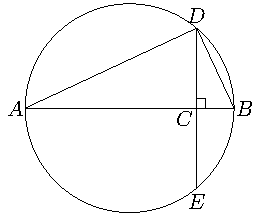
\includegraphics{221.png}
		\caption{}\label{aa}
	\end{figure}
	如图\ref{aa},$AB$时圆的直径,点$C$是$AB$上一点,$AC=a$,$BC=b$。过点$C$作垂直于$AB$的弦$DE$,连结$AD$,$BD$。容易证得$\bigtriangleup ACD \zhsimilar\bigtriangleup DCB$,因而$CD=\sqrt{ab}$。由于$CD$小于或等于圆的半径,用不等式表示为$\sqrt{ab}\leq\zfrac{a+b}{2}$。
	\par
	 显然,当且仅当点$C$与圆心重合,即当$a=b$时,上述不等式的等号成立。\par
	基本不等式的几何意义即为\tk{半弦长不大于半径长}。\par 
	基本不等式的常见变形式有:
	\begin{gather*}
	a+b\geq 2\sqrt{ab},
	ab\leq\Big(\zfrac{a+b}{2}\Big)^2.
	\end{gather*}
\end{multicols}
\lanmu{常考题型}
\begin{multicols}{2}
	\subsubsection{利用基本不等式求最值}
	\begin{liti}
		已知$x>0$,求$x+\zfrac{1}{x}$的最小值。
	\end{liti}
	\begin{jiexi}
		因为$x>0$,
		\[x+\zfrac{1}{x}\geq 2\sqrt{x\cdot\zfrac{1}{x}}=2,\]
		当且仅当$x=\zfrac{1}{x}$,即$x^2=1,x=1$时,等号成立,因此所求的最小值为2。
	\end{jiexi}
\begin{dianping}
	本例我们不仅明确了$\forall x>0$,有$x+\zfrac{1}{x}\geq 2$,而且给出了“当且仅当$x=\zfrac{1}{x}$,即$x^2=1,x=1$时,等号成立”,这是为了说明2是$x+\zfrac{1}{x}(x>0)$的一个取值。
\end{dianping}
\begin{liti}
	已知$x,y$都是正数,求证:
	\begin{enumerate}
		\item 如果积$xy$等于定值$P$,那么当$x=y$时,和$x+y$有最小值$2\sqrt{P}$;
		\item 如果和$x+y$等于定值$S$,那么当$x=y$时,积$xy$有最大值$\zfrac{1}{4}S^2$。
	\end{enumerate}
\end{liti}
\begin{zhengming}
	因为$x,y$都是正数,所以$\zfrac{x+y}{2}\geq\sqrt{xy}$。\par 
	(1)当积$xy$等于定值$P$时,$\zfrac{x+y}{2}\geq\sqrt{P}$,所以
	\[x+y\geq 2\sqrt{P},\]
	当且仅当$x=y$时,上式等号成立。于是,当$x=y$时,和$x+y$有最小值$2\sqrt{P}$。
	\par 
	(2)当和$x+y$等于定值$S$时,$\sqrt{xy}\leq\zfrac{S}{2}$,所以
	\[xy\leq\zfrac{1}{4}S^2,\]
	当且仅当$x=y$时,上式等号成立。于是,当$x=y$时,积$xy$有最大值$\zfrac{1}{4}S^2$。
\end{zhengming}
\begin{dianping}
		本例的内容称为最值定理,简记为:\bf{和定积最大,积定和最小。}
\end{dianping}
\begin{bslx}
	\item	当$x$取什么值时,$x^2+\zfrac{1}{x^2}$取得最小值?最小值是多少?
	\item 函数$y=2x(2-x)(0<x<2)$的最大值是
	\begin{xx}{$\zfrac{1}{4}$}{$\zfrac{1}{2}$}{1}{2}\end{xx}
	\item 设$a>1$,求$\zfrac{a^2}{a-1}$的最小值。
	\item 已知$a>b>0$,求$a^2+\zfrac{1}{b(a-b)}$的最小值。
\end{bslx}
\begin{ffgn}
	利用基本不等式求最值要牢记:{\bf 一正、二定、三相等}。\par 
	\quan{1}一正:各项必须为正。\par 
	\quan{2}二定:各项之和或各项之积为定值。\par 
	\quan{3}三相等:必须验证取等号时条件是否具备。
\end{ffgn}
	\subsubsection{利用基本不等式证明不等式}
\begin{liti}
	设$a>0,b>0$,求证:$\zfrac{a+b}{2}\leq\sqrt{\zfrac{a^2+b^2}{2}}$。
\end{liti}
\begin{zhengming}
	因为$a^2+b^2\geq 2ab$,所以\[2(a^2+b^2)\geq a^2+b^2+2ab=(a+b)^2,\]
	\begin{flalign*}
	&即&&\zfrac{a+b}{2}\leq\sqrt{\zfrac{a^2+b^2}{2}}.&&
	\end{flalign*}
	当且仅当$a=b$时,上式等号成立。
\end{zhengming}
\begin{dianping}
	我们把$\sqrt{\zfrac{a^2+b^2}{2}}$称为平方平均数。
\end{dianping}
\begin{liti}
	已知$a,b,c>0$,求证$\zfrac{a^2}{b}+\zfrac{b^2}{c}+\zfrac{c^2}{a}\geq a+b+c$。
\end{liti}
\begin{zhengming}
	因为$a,b,c>0$,由基本不等式得
	\begin{align*}
	&\zfrac{a^2}{b}+b\geq 2a,\tag*{\quan{1}}\\
	&\zfrac{b^2}{c}+c\geq 2b,\tag*{\quan{2}}\\
	&\zfrac{c^2}{a}+a\geq 2c,\tag*{\quan{3}}
	\end{align*}
	$\quan{1}+\quan{2}+\quan{3}$得
	\[\zfrac{a^2}{b}+\zfrac{b^2}{c}+\zfrac{c^2}{a}+a+b+c\geq 2a+2b+2c.\]
	故$\zfrac{a^2}{b}+\zfrac{b^2}{c}+\zfrac{c^2}{a}\geq a+b+c$,当且仅当$a=b=c$时,等号成立。
\end{zhengming}
\begin{dianping}
	本例$a,b,c$的地位一样,这样的式子叫做轮换对称式,合理地构造并正确选用基本不等式及其变形,是证明轮换对称结构的不等式的常用思路。
\end{dianping}
\begin{bslx}
	\item 设$a>0,b>0$,求证:\[\zfrac{2}{\zfrac{1}{a}+\zfrac{1}{b}}\leq \sqrt{ab}.\]
	\item 已知$a>0,b>0$,求证:\[a+b+1\geq\sqrt{ab}+\sqrt{a}+\sqrt{b}.\]
\end{bslx}
\begin{ffgn}
	利用基本不等式证明不等式时,要先观察题中要证明的不等式的结构特征,若不能直接使用基本不等式证明,则考虑对代数式进行拆项、变形、配凑等,使之转化为能使用基本不等式的形式。
\end{ffgn}
	\subsubsection{二元条件最值}
\begin{liti}
	设$x,y>0$,若$\zfrac{1}{x}+\zfrac{9}{y}=1$,则$x+y$的最小值是\tkt.
\end{liti}
\begin{jiexi}
	由题意\columnbreak
	\begin{align*}
	x+y&=(x+y)\left(\zfrac{1}{x}+\zfrac{1}{y}\right)\\
	&=10+\zfrac{y}{x}+\zfrac{9x}{y}\\
	&\geq10+2\sqrt{\zfrac{y}{x}\cdot\zfrac{9x}{y}}=16
	\end{align*}
	\par
	当且仅当
	\begin{equation*}
	\begin{dcases}
	\zfrac{y}{x}=\zfrac{9x}{y}\\
	\zfrac{1}{x}+\zfrac{9}{y}=1
	\end{dcases}
	\end{equation*}
	即$x=4,y=12$时取等号,所以$x+y$的最小值是16。
\end{jiexi}
\begin{dianping}
	本例解答过程中利用了“1”的代换。
\end{dianping}
\begin{bslx}
	\item 设$x,y>0$且$2x+3y=3$,则$\zfrac{3}{x}+\zfrac{2}{y}$的最小值是\tkt.
	\item 已知$a,b$是正实数,且$a+b=2$,求证:
	\begin{enumerate}
		\item $\sqrt{a}+\sqrt{b}\leq 2$;
		\item $(a+b^3)(a^3+b)\geq 4$.
	\end{enumerate}
\end{bslx}

\begin{ffgn}
	解题时为了挖掘出“积”或“和”为定值,常常需要根据题设条件采取合理配式、配系数的方法,创造条件正确地使用基本不等式。
\end{ffgn}
\end{multicols}
\lanmu{校本作业}
\begin{multicols}{2}
	\begin{zuoye}
		\item 已知实数$a>0,b>0$,且$2a+b=2ab$,则$a+2b$的最小值为\kuohao
		\begin{xx}{$\zfrac{5}{2}+\sqrt{2}$}{$\zfrac{9}{2}$}{$\zfrac{5}{2}$}{$4\sqrt{2}$}
			\end{xx}
		\item 若正实数$x,y$满足$x+y=1$,则$\zfrac{4}{x+1}+\zfrac{1}{y}$的最小值为\kuohao
		\begin{xx}{$\zfrac{44}{7}$}{$\zfrac{27}{5}$}{$\zfrac{14}{3}$}{$\zfrac{9}{2}$}
			\end{xx}
		\item 已知$x>0,y>0$,且$\zfrac{1}{x+1}+\zfrac{1}{y}=\zfrac{1}{2}$,则$x+y$的最小值为\kuohao
		\begin{xx}{3}{5}{7}{9}\end{xx}
		\item 已知正数$x,y,z$满足$x+y+z=1$,则$\zfrac{1}{x}+\zfrac{4}{y}+\zfrac{9}{z}$的最小值是\tkt.
		\item 一批救灾物资随51辆汽车从某市以$v \mathrm{km/h}$的速度匀速直达灾区,已知两地公路线长400km,为了安全起见,两辆汽车的间距不得小于$\zfrac{v^2}{800}$km,那么这批物资全部到达灾区,最少需要\tkt h.
		\item 已知$a,b\in\mathbb{R}$,且$a>b>0$,$a+b=1$,则$a^2+2b^2$的最小值为\tkt,$\zfrac{4}{a-b}+\zfrac{1}{2b}$的最小值为\tkt.
		\item 已知实数$a,b,c,d$满足$a+b=1,c+d=1$,则$\zfrac{1}{abc}+\zfrac{1}{c+d}$的最小值是\kuohao
		\begin{xx}{10}{9}{$4\sqrt{2}$}{$3\sqrt{3}$}\end{xx}
		\item 已知$a>0,b>0$,且$\zfrac{1}{a}+\zfrac{1}{b}=1$,则$4a+2b+\zfrac{b}{a}$的最小值等于\tkt.
		\item 已知实数$a>b>0$,且$a+b=2$,则$\zfrac{3a-b}{a^2+2ab-3b^2}$的最小值为\tkt.
		\item 在实数集$\mathbb{R}$中定义一种运算$*$,具有性质:
		\begin{enumerate}
			\item 对任意$a,b\in\mathbb{R}$,$a*b=b*a$;
			\item 对任意$a\in\mathbb{R}$,$a*0=a$;
			\item 对任意$a,b\in\mathbb{R}$,$(a*b)*c=c*(ab)+(a*c)+(b*c)-5c$。
		\end{enumerate}
		则函数$f(x)=x*\zfrac{1}{x}(x>0)$的最小值等于\tkt.
		\item 设$a,b,c$为三角形的三边,则三角形的面积$S$可由公式
		\[S=\sqrt{p(p-a)(p-b)(p-c)}\]
		求得,其中$p$为三角形周长的一半,这个公式被称为海伦—秦九韶公式。现有一个三角形的边长满足$a+b=12,c=8$,则此三角形面积的最大值为\kuohao
		\begin{xx}{$4\sqrt{5}$}{$4\sqrt{15}$}{$8\sqrt{5}$}{$8\sqrt{15}$}\end{xx}
	\end{zuoye}
\end{multicols}
\newpage
\section{不等式的解法}
\chapter{函数的概念与性质}
\section{函数的概念及其表示}
\subsection{函数的概念}
\subsection{函数的表示法}
\section{函数的基本性质}
\subsection{单调性与最大(小)值}
\subsection{奇偶性}
\section{幂函数}
\section{函数的应用(一)}
\chapter{指数函数与对数函数}
\section{指数}
\section{指数函数}
\section{对数}
\section{对数函数}
\section{函数的应用(二)}
\subsection{函数的零点与方程的解}
\subsection{用二分法求方程的近似解}
\subsection{函数模型的应用}
	\chapter{三角函数}
\section{任意角和弧度制}
\subsection{任意角}
\subsection{弧度制}
\section{三角函数的概念}
\subsection{三角函数的概念}
\subsection{同角三角函数的基本关系}
\section{三角函数}
\section{三角函数的图象与性质}
\subsection{正弦函数、余弦函数的图象}
\subsection{正弦函数、余弦函数的性质}
\subsection{正切函数的性质与图象}
\end{document}
